%=======================================================================
%  Póster 70 x 100 cm vertical — Proyectos REDD+ y deforestación municipal en
%  Colombia: un diseño escalonado con intensidad de tratamiento, 2001–2024
%
%  Compilar:  pdflatex poster.tex   (dos pasadas)
%  Requiere:  beamerposter, pgfplots, booktabs, tcolorbox
%  Figuras (copiar desde outputs/figuras/ a la carpeta del .tex):
%     47_event_study_linea_base.png      (47_linea_base_bootstrap.R)
%     43_leave_one_out.png              (43_robustez_anticipacion_y_loo.R)
%     42_dosis_vs_att_relativo.png      (42_pendiente_dosis_manual.R)
%=======================================================================
\documentclass[final,t]{beamer}
% Formato de impresión 70 x 100 cm. Todas las medidas absolutas (cm y
% \fontsize) están escaladas por 70/84,1 = 0,832 respecto de la versión A0.
% scale=0.79 (y no 0,97 x 0,832 = 0,81): beamerposter redondea los tamaños de
% letra y con 0,81 el contenido desborda la página.
\usepackage[orientation=portrait,size=custom,width=70,height=100,scale=0.79]{beamerposter}
\usepackage[utf8]{inputenc}
\usepackage[T1]{fontenc}
\usepackage{helvet}
\renewcommand{\familydefault}{\sfdefault}
\usepackage{anyfontsize}
\usepackage{colortbl}
\usepackage{booktabs}
\usepackage{tabularx}
\usepackage{ragged2e}
\usepackage{amsmath}
\usepackage{amssymb}
\usepackage{graphicx}
\usepackage{tcolorbox}
\usepackage{pgfplots}
\pgfplotsset{compat=1.18}
\tcbuselibrary{skins}

%----------------------- Paleta -----------------------
\definecolor{tinta}{HTML}{12261E}
\definecolor{dosel}{HTML}{1D4F3F}
\definecolor{papel}{HTML}{F2F4EF}
\definecolor{reduccion}{HTML}{2F7A5B}
\definecolor{brasa}{HTML}{8F3B1F}
\definecolor{amazonia}{HTML}{B8860F}
\definecolor{regla}{HTML}{C4CEC6}
\definecolor{tenue}{HTML}{5B6E63}
\definecolor{cajafondo}{HTML}{E6EBE4}
\definecolor{alertafondo}{HTML}{F4E7E0}
\definecolor{politicafondo}{HTML}{E4EFE7}
\definecolor{orofondo}{HTML}{F6ECD2}

%----------------------- Tema -------------------------
\usetheme{default}
\usecolortheme{default}
\setbeamercolor{background canvas}{bg=papel}
\setbeamercolor{normal text}{fg=tinta}
\setbeamercolor{block title}{bg=papel,fg=dosel}
\setbeamercolor{block body}{bg=papel,fg=tinta}
\setbeamerfont{block title}{series=\bfseries,size=\Large}
\setbeamertemplate{navigation symbols}{}
\setbeamertemplate{caption}[numbered]
\setbeamerfont{caption}{size=\small}
\setbeamercolor{caption name}{fg=tenue}
\setbeamercolor{itemize item}{fg=reduccion}
\setbeamertemplate{itemize item}{\raisebox{0.18ex}{\rule{0.45ex}{0.45ex}}}
\setlength{\parskip}{0.4\baselineskip}

% Título de sección con filete y referencia al capítulo de la tesis
\newcommand{\seccion}[2]{%
  \par\vspace{0.5\baselineskip}%
  {\color{dosel}\Large\bfseries #1\hfill{\color{tenue}\normalsize\mdseries #2}}\par
  \vspace{-0.35\baselineskip}%
  {\color{dosel}\rule{\linewidth}{2.2pt}}\par
  \vspace{0.25\baselineskip}%
}

% Nota de pie, cuerpo pequeño
\newcommand{\nota}[1]{{\color{tenue}\small #1\par}}

% Numeración propia del póster (Tabla 1..n, Figura 1..n), en orden de lectura.
% Se usa \ref para las remisiones internas: compilar dos veces.
\newcounter{figposter}
\newcounter{tabposter}
\newcommand{\figcap}[2]{\refstepcounter{figposter}\label{#1}%
  \nota{\textbf{Figura~\thefigposter.} #2}}
\newcommand{\tabcap}[2]{\refstepcounter{tabposter}\label{#1}%
  \nota{\textbf{Tabla~\thetabposter.} #2}}

% Cifra destacada
\newcommand{\cifra}[2]{%
  \parbox[t]{0.46\linewidth}{%
    {\color{tinta}\rule{\linewidth}{2.5pt}}\\[0.25\baselineskip]
    {\color{dosel}\fontsize{42}{43}\selectfont\bfseries #1}\\[0.2\baselineskip]
    {\color{tenue}\small #2}}%
}

% Caja de contenido
\newtcolorbox{caja}[2][cajafondo]{
  colback=#1, colframe=dosel, boxrule=0pt, leftrule=5pt,
  sharp corners, left=8pt, right=8pt, top=8pt, bottom=8pt,
  title=\textbf{#2}, coltitle=tinta, fonttitle=\large,
  attach title to upper=\par\vspace{2mm}
}

\begin{document}
\begin{frame}[t]{}

%=======================================================================
%  CABECERA
%=======================================================================
\begin{tcolorbox}[colback=dosel,colframe=dosel,boxrule=0pt,sharp corners,
  left=0.999cm,right=0.999cm,top=0.832cm,bottom=0.832cm]
  {\color{papel!70}\normalsize Maestría en Economía Aplicada \quad\textbullet\quad Tesis de grado
   \hfill Entidad destinataria: Ministerio de Ambiente y Desarrollo Sostenible (MADS)}\\[0.25cm]
  {\color{papel!40}\rule{\linewidth}{1pt}}\\[0.499cm]
  {\color{papel}\fontsize{60}{67}\selectfont\bfseries
   Proyectos REDD+ y deforestación municipal en Colombia:}\\[0.291cm]
  {\color{papel!80}\fontsize{42}{48}\selectfont\bfseries
   un diseño escalonado con intensidad de tratamiento, 2001--2024}\\[0.583cm]
  {\color{papel!85}\large\textbf{José David Cuervo Urrego}\quad\textbullet\quad
   \textbf{Harold Stiven Acuña Alaguna}\qquad Asesor: Jorge Luis Montero Mestre}
\end{tcolorbox}



%=======================================================================
%  FRANJA: HALLAZGO PRINCIPAL
%=======================================================================
\begin{tcolorbox}[colback=tinta,colframe=tinta,boxrule=0pt,sharp corners,
  left=0.999cm,right=0.999cm,top=0.749cm,bottom=0.749cm]
\begin{minipage}[c]{0.36\linewidth}
  {\color{papel}\fontsize{33}{38}\selectfont\bfseries El signo depende de la línea base}\\[0.499cm]
  \setlength{\leftskip}{0.749cm}\setlength{\parindent}{-0.749cm}
  \color{papel!75}\large
  \textcolor{amazonia}{\rule{0.45ex}{0.45ex}}\hspace{0.416cm}Contra el año previo a la adopción ($g-1$),
  negativo con Callaway--Sant'Anna y Sun--Abraham, pero
  \textbf{\textcolor{amazonia}{ningún intervalo excluye el cero}}.\par\vspace{0.291cm}
  \textcolor{amazonia}{\rule{0.45ex}{0.45ex}}\hspace{0.416cm}$g-1$ es un año alto: con base $g-2$ el efecto
  cae 60\,\%, y contra \textbf{\textcolor{amazonia}{todos los años previos}} (Wooldridge) pasa a
  $+$211~ha.\par\vspace{0.291cm}
  \textcolor{amazonia}{\rule{0.45ex}{0.45ex}}\hspace{0.416cm}Ninguna exclusión individual cambia el signo,
  pero \textbf{\textcolor{amazonia}{tres de 37 municipios}} sostienen casi todo el estimado puntual.\par
\end{minipage}\hfill
\begin{minipage}[c]{0.60\linewidth}
\centering
\begin{tikzpicture}[x=0.015cm,y=0.832cm,
   nombre/.style={anchor=east,align=right,text width=10.404cm,text=papel!75,font=\normalsize},
   sub/.style={anchor=east,align=right,text width=10.404cm,text=papel!50,font=\small},
   valor/.style={anchor=west,font=\bfseries\normalsize},
   eje/.style={anchor=north,text=papel!50,font=\normalsize}]
  % rejilla vertical
  \foreach \v in {-1000,-750,-500,-250,250,500}
    \draw[papel!22,very thin] (\v,0.7) -- (\v,-9.10);
  \draw[papel!65,dashed,semithick] (0,0.85) -- (0,-9.25);
  % --- Callaway--Sant'Anna (principal), DR, base $g-1$ ---
  \node[nombre] at (-1090,0.27) {Callaway--Sant'Anna (principal)};
  \node[sub]    at (-1090,-0.45) {DR, base $g-1$};
  \draw[amazonia,thick] (-1029.25,0.00) -- (99.47,0.00);
  \fill[amazonia] (-464.89,-0.28) rectangle (0,0.28);
  \node[valor,text=amazonia!70] at (114,0.00) {$-$464{,}9};
  % --- Sun--Abraham, base $g-1$ ---
  \node[nombre] at (-1090,-1.13) {Sun--Abraham};
  \node[sub]    at (-1090,-1.85) {base $g-1$};
  \draw[amazonia!80,semithick] (-759.4,-1.40) -- (57.7,-1.40);
  \fill[amazonia!70] (-324.9,-1.68) rectangle (0,-1.12);
  \node[valor,text=amazonia!55] at (73,-1.40) {$-$324{,}9};
  % --- Callaway--Sant'Anna, base $g-2$ ---
  \node[nombre] at (-1090,-2.53) {Callaway--Sant'Anna};
  \node[sub]    at (-1090,-3.25) {base $g-2$};
  \draw[reduccion!80,semithick] (-654.93,-2.80) -- (285.78,-2.80);
  \fill[reduccion!85] (-184.58,-3.08) rectangle (0,-2.52);
  \node[valor,text=reduccion!45] at (301,-2.80) {$-$184{,}6};
  % --- Callaway--Sant'Anna, base $g-3$ ---
  \node[nombre] at (-1090,-3.93) {Callaway--Sant'Anna};
  \node[sub]    at (-1090,-4.65) {base $g-3$};
  \draw[reduccion!80,semithick] (-923.51,-4.20) -- (355.98,-4.20);
  \fill[reduccion!85] (-283.77,-4.48) rectangle (0,-3.92);
  \node[valor,text=reduccion!45] at (371,-4.20) {$-$283{,}8};
  % --- Wooldridge, base = todos los años previos ---
  \node[nombre] at (-1090,-5.33) {Wooldridge};
  \node[sub]    at (-1090,-6.05) {base = todos los años previos};
  \draw[brasa!45!papel,semithick] (-98.84,-5.60) -- (544.91,-5.60);
  \fill[brasa!55!papel] (0,-5.88) rectangle (211.02,-5.32);
  \node[valor,text=brasa!35!papel] at (560,-5.60) {$+$211{,}0};
  % --- Sin Cartagena del Chairá, 1 de 37 tratados ---
  \node[nombre] at (-1090,-6.73) {Sin Cartagena del Chairá};
  \node[sub]    at (-1090,-7.45) {1 de 37 tratados};
  \draw[reduccion!80,semithick] (-737.15,-7.00) -- (206.45,-7.00);
  \fill[reduccion!85] (-265.35,-7.28) rectangle (0,-6.72);
  \node[valor,text=reduccion!45] at (221,-7.00) {$-$265{,}4};
  % --- Sin los tres más influyentes, prueba de estrés, ver Fig.~\ref{fig:loo} ---
  \node[nombre] at (-1090,-8.13) {Sin los tres más influyentes};
  \node[sub]    at (-1090,-8.85) {prueba de estrés, ver Fig.~\ref{fig:loo}};
  \draw[papel!55,semithick] (-466.43,-8.40) -- (452.11,-8.40);
  \fill[papel!55] (-7.16,-8.68) rectangle (0,-8.12);
  \node[valor,text=papel!60] at (467,-8.40) {$-$7{,}2};
  % --- escala ---
  \foreach \v/\t in {-1000/$-$1.000,-750/$-$750,-500/$-$500,-250/$-$250,0/0,250/$+$250,500/$+$500}
    \node[eje] at (\v,-9.20) {\t};
  \node[anchor=north,text=papel!50,font=\normalsize] at (-250,-10.05)
    {ATT promedio $e=0,\dots,5$ sobre pérdida anual de bosque (ha) \textbullet\ línea = IC 95\,\%};
\end{tikzpicture}

\vspace{0.25cm}
\refstepcounter{figposter}\label{fig:franja}%
{\color{papel!60}\small\textbf{Figura~\thefigposter.} Sensibilidad del ATT al estimador, a la línea base y a la
exclusión de municipios influyentes. IC de SA y Wooldridge: bootstrap de municipios por cohorte.\par}
\end{minipage}
\end{tcolorbox}



%=======================================================================
%  TRES COLUMNAS
%=======================================================================
\begin{columns}[t]

%-------------------- COLUMNA 1 --------------------
\begin{column}{0.305\paperwidth}
\justifying

\seccion{Problema de política}{}
\begin{itemize}
  \item El mecanismo de no causación (Ley 1819 de 2016, Decreto 926 de 2017) permite compensar
        el impuesto al carbono con créditos certificados.
  \item Ese incentivo aceleró la expansión de proyectos REDD+ sin evaluación causal previa.
  \item[\textcolor{brasa}{\rule{0.45ex}{0.45ex}}] Sobreacreditación documentada: los créditos emitidos
        equivalen a \textbf{10,7 veces} las reducciones verificables en 44 proyectos REDD+
        (Swinfield et al., 2026).
  \item Sin evidencia causal, el MADS no distingue beneficio climático real de acreditación
        no atribuible.
\end{itemize}

\vspace{0.25cm}
{\color{amazonia}\rule{3pt}{2.164cm}}\hspace{0.333cm}%
\begin{minipage}[b]{0.88\linewidth}
  {\color{dosel}\fontsize{25}{30}\selectfont\itshape
   ¿Cuál es el efecto causal de la implementación de proyectos REDD+ sobre la
   deforestación en los municipios colombianos?}
\end{minipage}

\vspace{0.28cm}
\nota{Se evalúa la \textbf{intervención territorial}, no el crédito ni la certificación: bonos de
carbono no es sinónimo de REDD+. Ninguno de los 12 proyectos de Gold Standard en Colombia es
REDD+, y de los REDD+ de Verra solo 13 están registrados.}

\seccion{Datos}{}
\cifra{1.122}{municipios}\hfill\cifra{26.928}{observaciones municipio año}

\vspace{0.416cm}
\cifra{43}{municipios tratados REDD+ (depurado)}\hfill\cifra{37}{tratados en la ventana de cohortes 2013 - 2019}

\vspace{0.30cm}
\textbf{\large Resultado}
\begin{itemize}
  \item Pérdida de cobertura arbórea, Global Forest Change a 30~m (Hansen et al., 2013),
        por estadística zonal.
  \item Distribución muy asimétrica: mediana de 22~ha frente a máximos sobre 30.000~ha
        $\rightarrow$ se reporta también el efecto \textbf{relativo} a la deforestación
        propia de 2001--2012.
\end{itemize}

\textbf{\large Tratamiento}
\tabcap{tab:registros}{Registros consultados y método de asignación municipal.}
\begin{center}
\begin{tabularx}{\linewidth}{Xrl}
\toprule
\rowcolor{dosel}
\textcolor{papel}{\textbf{Registro}} & \textcolor{papel}{\textbf{Proy.}} &
\textcolor{papel}{\textbf{Asignación}}\\
\midrule
Verra (API Platts/S\&P) & 101 & Punto en polígono\\
Gold Standard (API)     & 28  & Punto en polígono\\
RENARE (MADS)           & 281 & Coincidencia textual\\
Cercarbono (Excel)      & 234 & Coincidencia textual\\
OffsetsDB               & 270 & Solo descubrimiento\\
\bottomrule
\end{tabularx}
\end{center}
\nota{Filtro REDD+ por campo estructurado (metodologías VM0006, VM0007, VM0009, VM0015 y actividad
AFOLU), no por nombre del proyecto: 82 eventos en 50 municipios.}

\begin{caja}{Depuración del tratamiento}
\begin{itemize}
  \item \textbf{Geocodificación:} se excluye CO2ROZO, 400.000~ha ubicadas en la sede del proponente
        (Barranquilla).
  \item \textbf{Estado de registro:} 6 municipios cuyo único vínculo REDD+ es un proyecto
        retirado o rechazado salen de la muestra; \textbf{no pasan a control}.
  \item La cohorte la fija el proyecto vivo: Mitú pasa de 2017 a 2018.
  \item[\textcolor{amazonia}{\rule{0.45ex}{0.45ex}}] De 48 a 43 tratados. El ATT se mueve 9\,\%:
        el resultado es robusto a la depuración.
\end{itemize}
\end{caja}

\seccion{Hipótesis y contraste}{}
\tabcap{tab:hipotesis}{Hipótesis de la tesis y veredicto empírico.}
\begin{center}
\begin{tabularx}{\linewidth}{lX}
\toprule
\rowcolor{dosel}
\textcolor{papel}{\textbf{Hipótesis}} & \textcolor{papel}{\textbf{Veredicto empírico}}\\
\midrule
H1. ATT negativo           & Negativo contra $g-1$, positivo contra todo el previo, ningún IC excluye el cero\\
H2. Sin dinámicas previas  & Rechazada: $g-1$ es un año alto, $\bar{M}$ de ruptura $=0$\\
H3. Efecto persistente     & Sin precisión para afirmarlo\\
H4. Fuga hacia vecinos     & Sin fuga detectable: $-$59~ha, IC [$-$221 ; 102] (DR, 108 vecinos expuestos)\\
H5. Mayor efecto a mayor intensidad & Sin gradiente identificable\\
\bottomrule
\end{tabularx}
\end{center}

\end{column}

%-------------------- COLUMNA 2 --------------------
\begin{column}{0.305\paperwidth}
\justifying

\seccion{Estrategia empírica}{}
\nota{Diferencias en diferencias con adopción escalonada (Callaway y Sant'Anna, 2021),
identificado contra el año previo a la adopción:}
\begin{tcolorbox}[colback=cajafondo,colframe=regla,boxrule=0.8pt,sharp corners]
\centering
\[
  ATT(g,t) \;=\; \mathbb{E}\!\left[Y_{t}-Y_{g-1}\,\middle|\,G_{g}=1\right]
               \;-\; \mathbb{E}\!\left[Y_{t}-Y_{g-1}\,\middle|\,C=1\right]
\]
\raggedright\nota{$G_g$: cohorte que adopta en el año $g$. $C$: municipios aún no tratados.}
\end{tcolorbox}

\nota{Intensidad de tratamiento continua (Callaway, Goodman-Bacon y Sant'Anna, 2024):}
\begin{tcolorbox}[colback=cajafondo,colframe=regla,boxrule=0.8pt,sharp corners]
\centering
\[
  ATT(d) \;=\; \mathbb{E}\!\left[\Delta Y \,\middle|\, D=d\right]
         \;-\; \mathbb{E}\!\left[\Delta Y \,\middle|\, D=0\right]
\]
\raggedright\nota{La pendiente $\partial ATT(d)/\partial d$ solo es causal bajo tendencias
paralelas \emph{fuertes}: que municipios de distinta dosis respondan igual a la misma dosis.}
\end{tcolorbox}

\begin{itemize}
  \item Doblemente robusto con \textbf{diez covariables} de línea base: clima, accesibilidad,
        conflicto, coca, deforestación previa y su tendencia.
  \item Cohortes 2013 - 2019; los tratados fuera de la ventana salen de la muestra.
  \item Robustez: estimadores de Sun y Abraham (2021) y Wooldridge (2021), año base
        (anticipación), exclusión uno a uno, D1 sin depurar y sensibilidad de Rambachan y Roth (2023) a violaciones de tendencias paralelas.
\end{itemize}

\seccion{Efecto promedio}{}
\tabcap{tab:att}{ATT simple sobre la pérdida de bosque, cohortes 2013 - 2019. Relativo: ATT sobre
la media pretratamiento de los tratados.}
\begin{center}
\begin{tabularx}{\linewidth}{Xrrr}
\toprule
\rowcolor{dosel}
\textcolor{papel}{\textbf{Especificación}} & \textcolor{papel}{\textbf{ATT (ha)}} &
\textcolor{papel}{\textbf{EE}} & \textcolor{papel}{\textbf{Rel.}}\\
\midrule
\rowcolor{orofondo}
\textbf{Depurada · DR (principal)} & \textcolor{reduccion}{\textbf{$-$424,99}} & 263,82 & $-$43\,\%\\
Depurada · sin covariables & \textcolor{reduccion}{\textbf{$-$176,87}} & 298,25 & $-$18\,\%\\
Sin depurar · DR           & \textcolor{reduccion}{\textbf{$-$388,61}} & 208,43 & $-$39\,\%\\
\bottomrule
\end{tabularx}
\end{center}
\begin{itemize}
  \item IC 95\,\% de la principal: [$-$942 ; 92] ha.
  \item[\textcolor{brasa}{\rule{0.45ex}{0.45ex}}] Sin covariables el efecto cae a menos de la mitad:
        la comparación incondicional contra el promedio nacional es débil.
\end{itemize}

\seccion{Año base y tendencias previas}{}
\begin{center}
% trim: recorta la leyenda del PNG (los símbolos se explican en el pie)
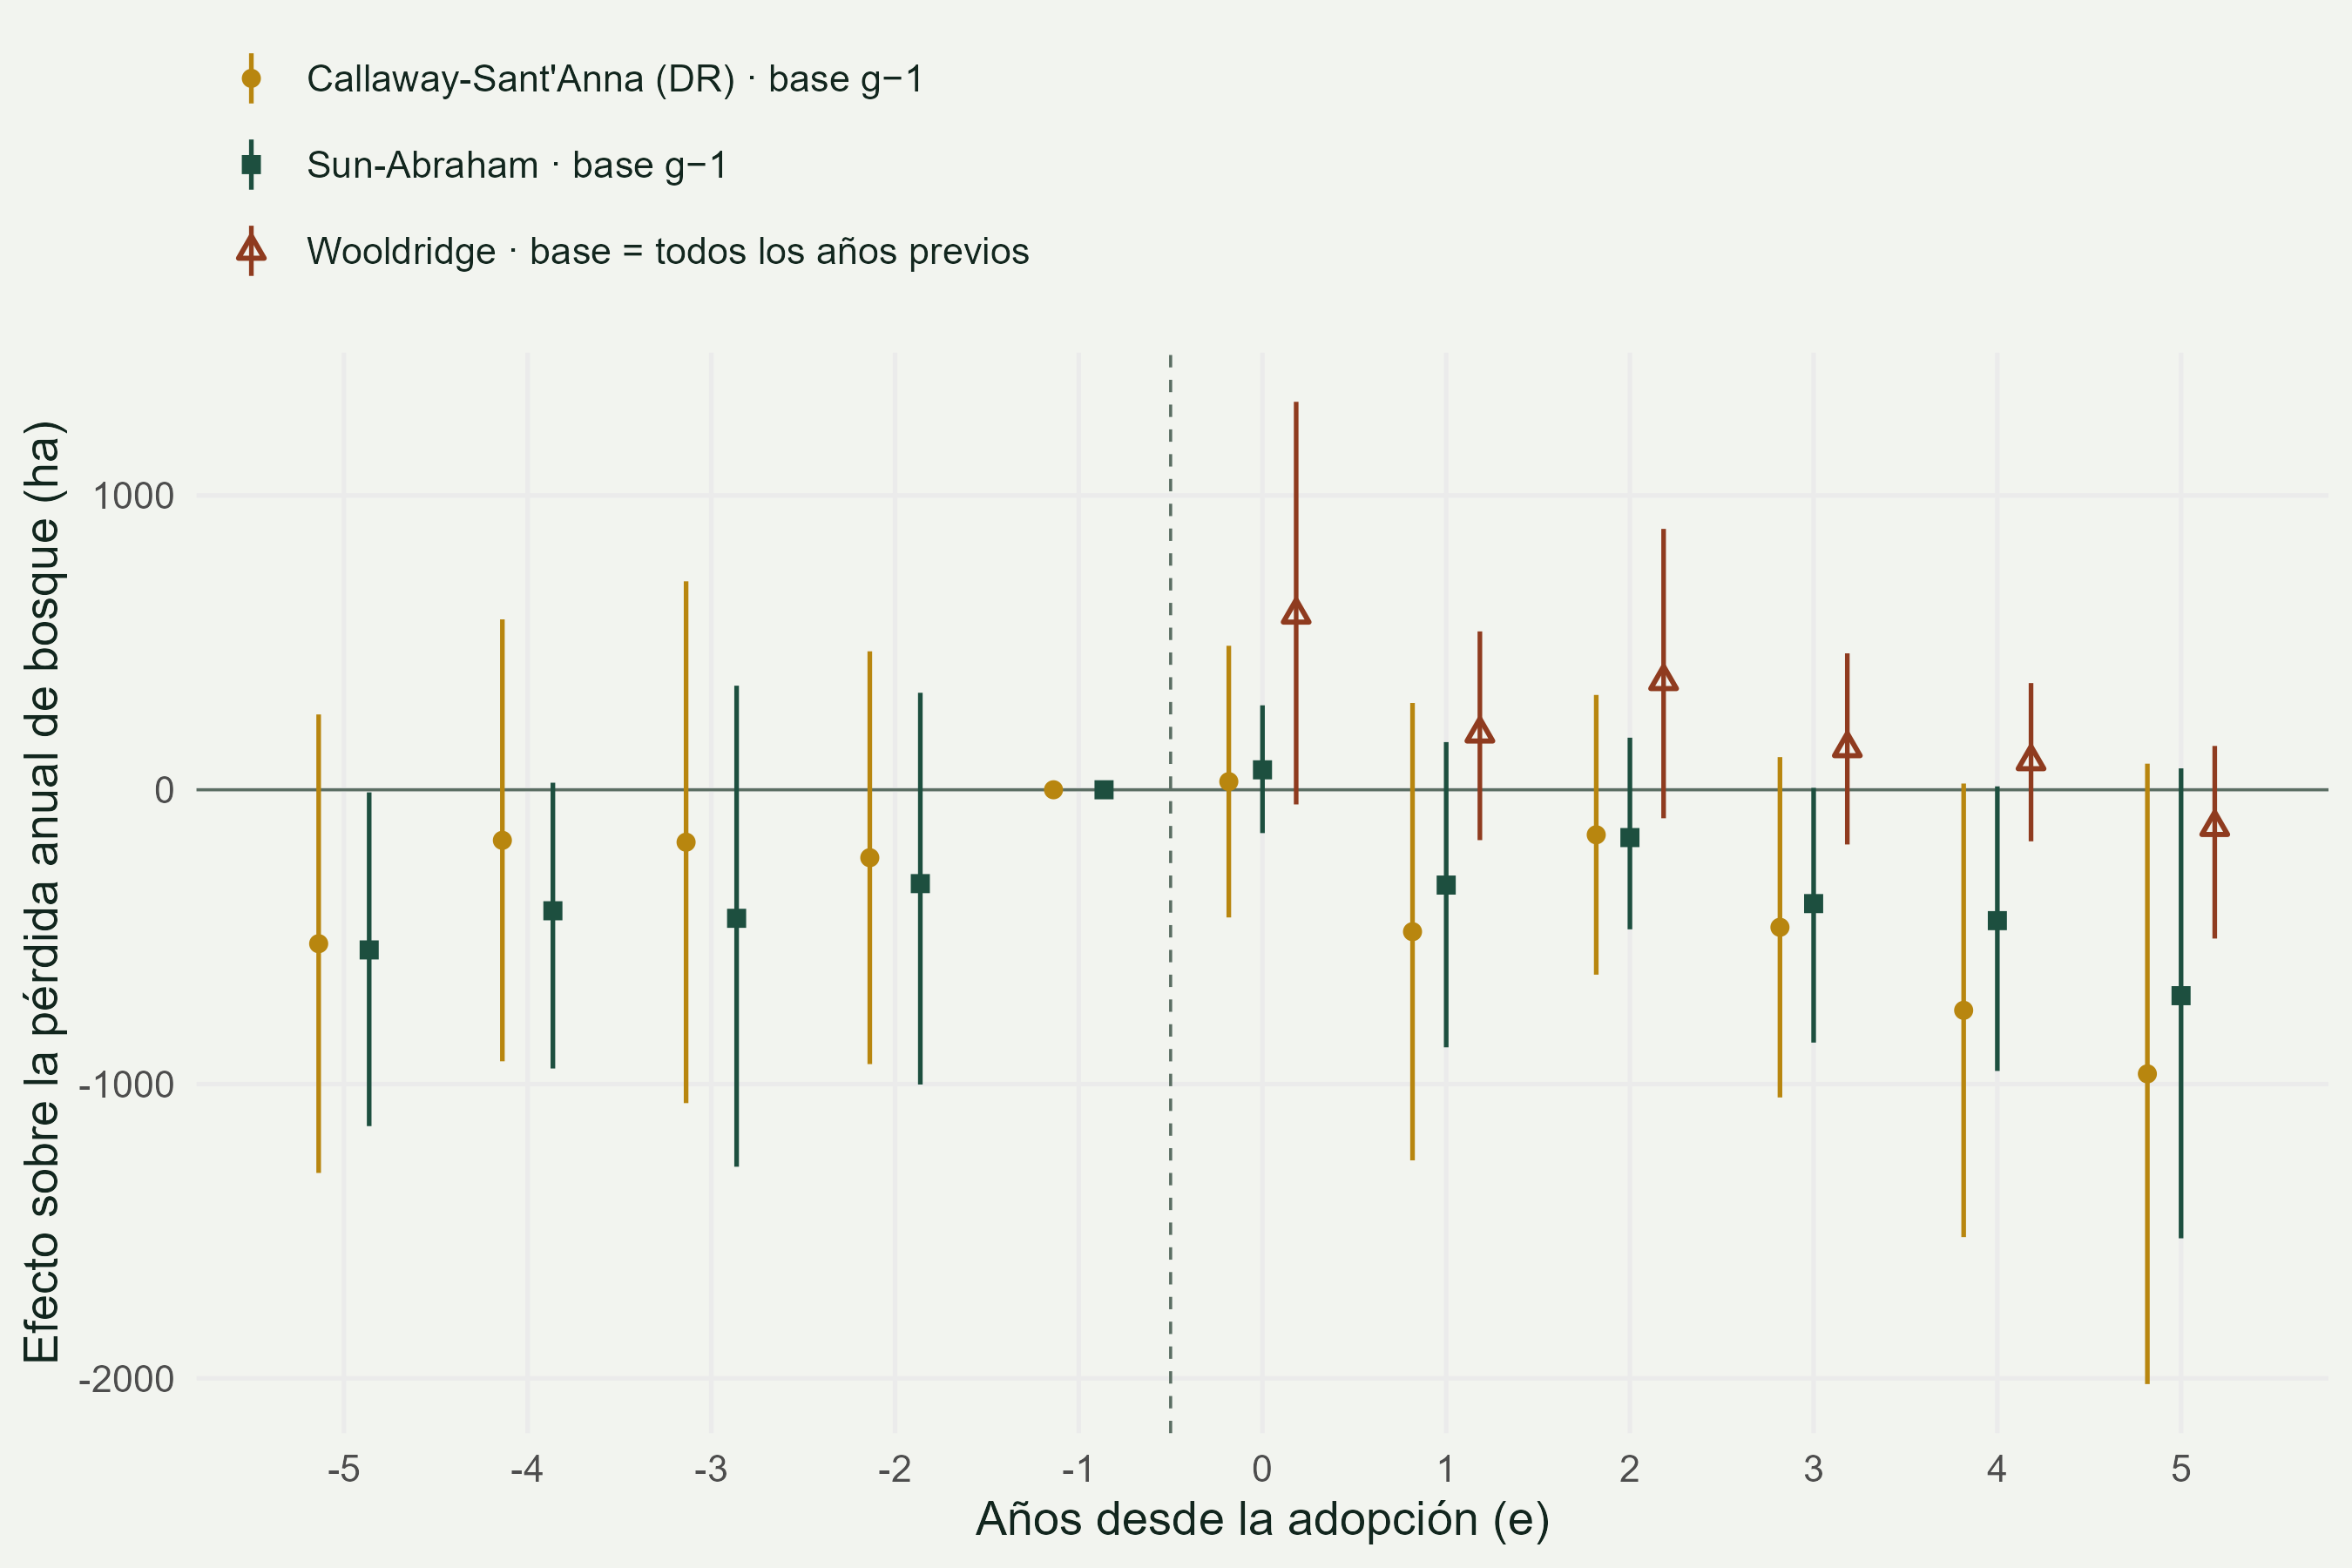
\includegraphics[width=0.86\linewidth,trim=0 0 0 82,clip]{47_event_study_linea_base.png}
\end{center}
\figcap{fig:es}{Estudio de eventos con tres estimadores robustos a efectos heterogéneos.
\textcolor{amazonia}{$\bullet$} Callaway y Sant'Anna (2021, DR) y \textcolor{dosel}{$\blacksquare$}
Sun y Abraham (2021), contra $g-1$; \textcolor{brasa}{$\triangle$} Wooldridge (2021), contra el
promedio de todos los años previos (con controles nunca tratados coincide con Sun--Abraham).
IC 95\,\%: bootstrap multiplicador (CS) y de municipios por cohorte, $B=499$.}
\begin{itemize}
  \item Contra $g-1$: $-$465 (CS) y $-$325~ha (SA, IC [$-$759 ; 58]), con previos negativos en
        ambos: \textbf{$g-1$ es un año alto}.
  \item[\textcolor{amazonia}{\rule{0.45ex}{0.45ex}}] Contra todos los años previos, Wooldridge da
        \textbf{$+$211~ha} (IC [$-$99 ; 545]). La distancia entre triángulos y cuadrados es el
        efecto del año base.
  \item Un pico en $g-1$ sesga hacia un efecto negativo; una tendencia previa creciente, hacia uno
        positivo. Rambachan y Roth: $\bar{M}$ de ruptura $=0$.
\end{itemize}

\seccion{Influencia por municipio}{}
\begin{center}
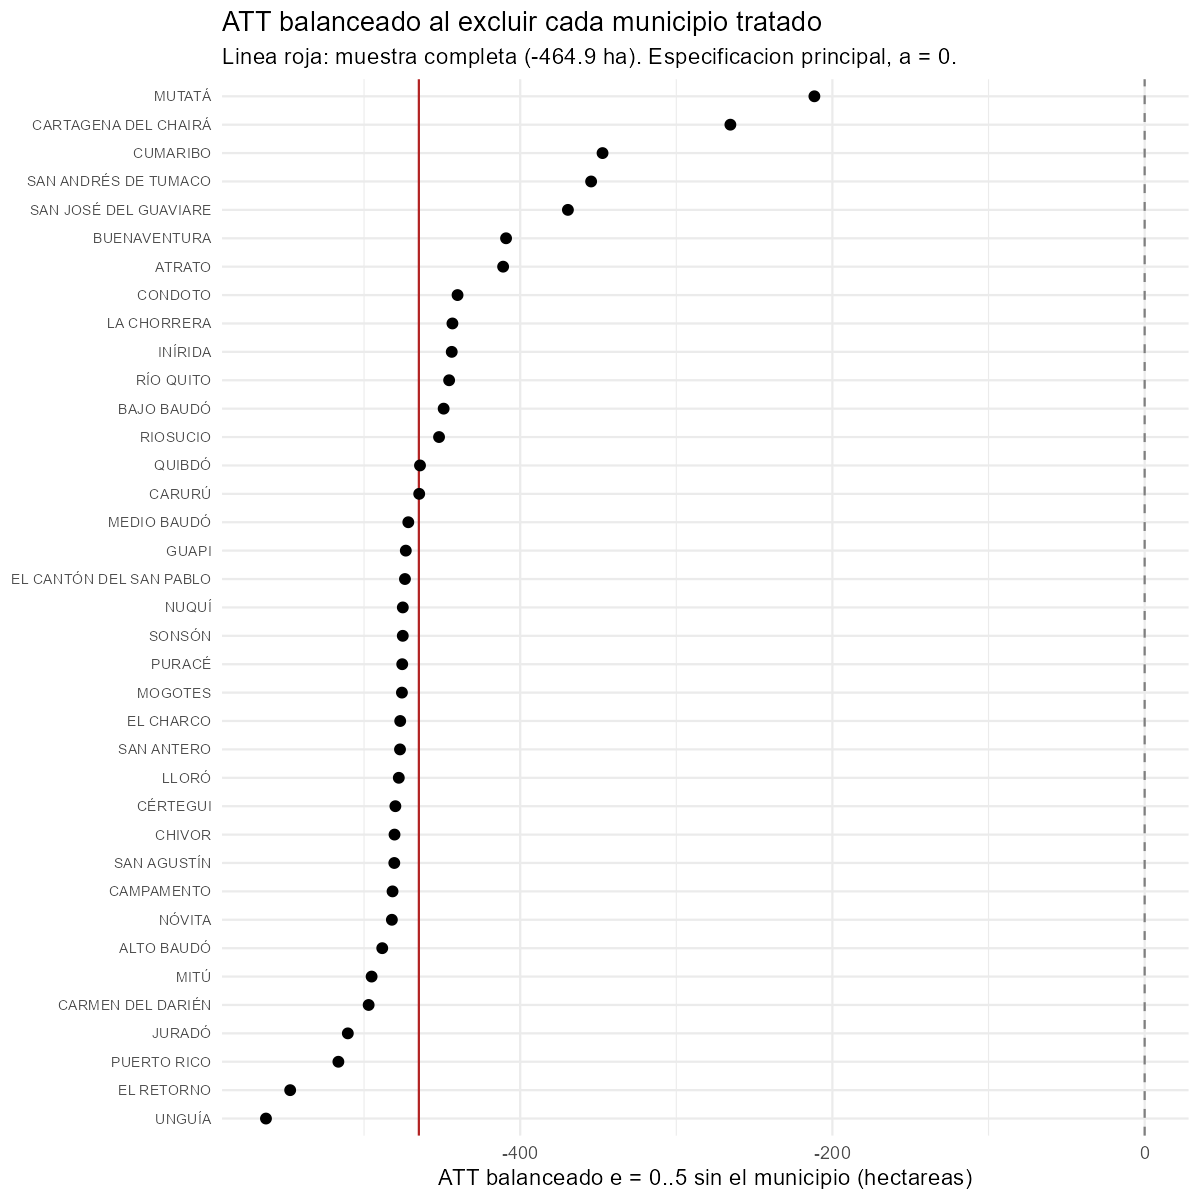
\includegraphics[width=0.60\linewidth]{43_leave_one_out.png}
\end{center}
\figcap{fig:loo}{ATT balanceado al excluir cada uno de los 37 tratados. Rango: [$-$563 ; $-$212]~ha.}

\end{column}

%-------------------- COLUMNA 3 --------------------
\begin{column}{0.305\paperwidth}
\justifying

\seccion{Intensidad del tratamiento}{}
\nota{Dos medidas pedidas por la dirección, con área declarada del proyecto $a_p$ y bosque base
$F_i^{2000}$ (dosel $\geq$30\,\%, validado contra Earth Engine):}
\begin{tcolorbox}[colback=cajafondo,colframe=regla,boxrule=0.8pt,sharp corners]
\centering
\[
  D_i^{\text{área}} = \frac{\sum_{p\in P_i} a_p}{A_i}
  \qquad\qquad
  D_i^{\text{bosque}} = \frac{\sum_{p\in P_i} a_p}{F_i^{2000}}
\]
\end{tcolorbox}
\cifra{29 de 43}{tratados con área publicada}\hfill\cifra{0,97}{correlación entre las dos medidas}

\vspace{0.166cm}
\tabcap{tab:terciles}{ATT por tercil de $D^{\text{bosque}}$, estudio de eventos balanceado, relativo a la
media pretratamiento de cada tercil.}
\begin{center}
\begin{tabularx}{\linewidth}{Xrrrr}
\toprule
\rowcolor{dosel}
\textcolor{papel}{\textbf{Tercil}} & \textcolor{papel}{\textbf{$n$}} &
\textcolor{papel}{\textbf{Media pre}} & \textcolor{papel}{\textbf{Sin cov.}} &
\textcolor{papel}{\textbf{DR}}\\
\midrule
Bajo  & 9 & 2.191~ha & $-$28\,\% & $-$41\,\%\\
Medio & 9 &   522~ha & $+$8\,\%  & $-$7\,\%\\
Alto  & 7 &   114~ha & $-$33\,\% & $-$1\,\%\\
\bottomrule
\end{tabularx}
\end{center}
\nota{En hectáreas, el tercil bajo parecía el más efectivo: su deforestación base es 19 veces la
del alto. Normalizado, no hay gradiente monótono.}

\begin{center}
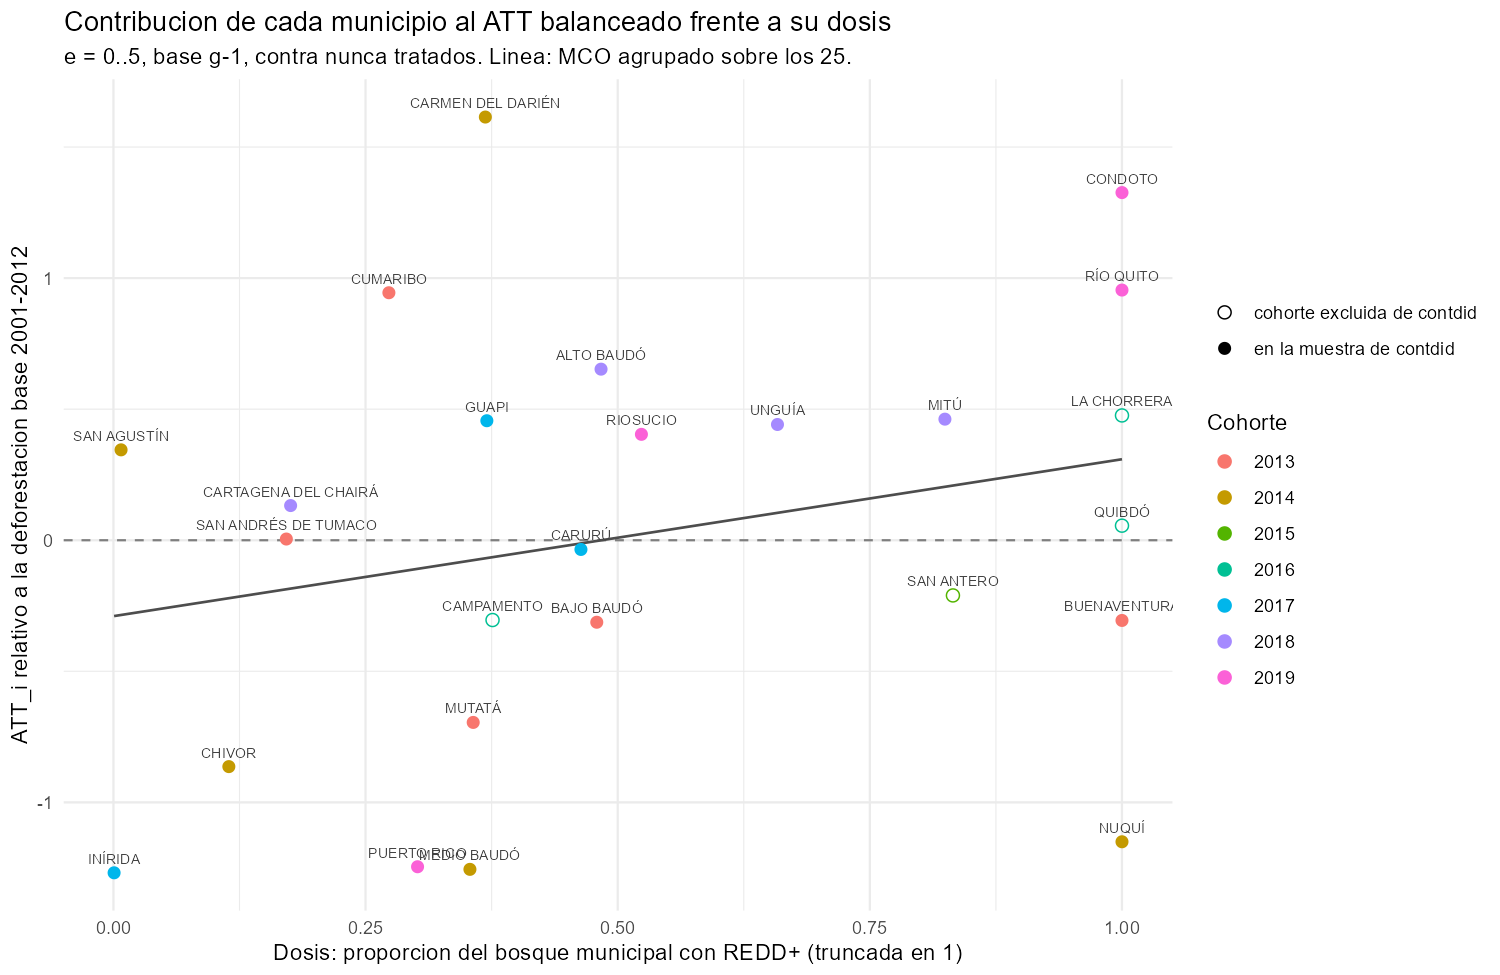
\includegraphics[width=0.96\linewidth]{42_dosis_vs_att_relativo.png}
\end{center}
\figcap{fig:dosis}{Contribución de cada municipio al ATT frente a su dosis, escala relativa.}

\tabcap{tab:pendiente}{Pendiente de la relación dosis--efecto según método y año base.}
\begin{center}
\begin{tabularx}{\linewidth}{Xrl}
\toprule
\rowcolor{dosel}
\textcolor{papel}{\textbf{Pendiente}} & \textcolor{papel}{\textbf{Punto}} &
\textcolor{papel}{\textbf{Inferencia}}\\
\midrule
\textit{contdid} 0.1.1       & 0,76     & EE 0,0009: subestimado\\
Manual, base $g-1$           & 0,60     & IC [$-$0,20 ; 1,39]; $p$ = 0,22\\
Manual, base $g-5\dots g-1$  & $-$0,05  & cambia de signo\\
\bottomrule
\end{tabularx}
\end{center}
\nota{Descomposición exacta del ATT por municipio; bootstrap estratificado de tratados y controles,
y permutación de la dosis.}

\begin{caja}[alertafondo]{Por qué no hay curva dosis-respuesta}
\begin{itemize}
  \item Entre 21 y 25 municipios con variación de dosis suficiente.
  \item Un tercio de las dosis \textbf{censuradas en 1}: los proyectos grandes cruzan fronteras
        municipales y el área declarada excede la del municipio anfitrión.
  \item La pendiente depende del año base: no está identificada.
\end{itemize}
\end{caja}

\begin{caja}[orofondo]{El salto previo tiene lectura de política}
Si los proyectos se instalan tras un pico de deforestación, el DiD atribuye al proyecto el retorno
a la normalidad, y la línea base del proyecto incorpora ese pico e infla los créditos. Es el
mecanismo de sobreacreditación documentado para REDD+ voluntario (West et al., 2020; 2023): el
sesgo que complica la identificación es el mismo que compromete la integridad de los créditos.
El salto previo aparece también en los municipios vecinos: la presión es regional.
\end{caja}

\seccion{Limitaciones}{}
\begin{itemize}
  \item[\textcolor{brasa}{\rule{0.45ex}{0.45ex}}] Sin polígonos: la dosis suma áreas declaradas
        (no su unión) y las asigna al municipio anfitrión.
  \item[\textcolor{brasa}{\rule{0.45ex}{0.45ex}}] Cercarbono y RENARE no publican área ni estado de
        registro: 14 tratados sin dosis.
  \item[\textcolor{brasa}{\rule{0.45ex}{0.45ex}}] Se mide pérdida de cobertura arbórea, no de bosque
        natural; la salida de las FARC-EP desde 2016 es explicación alternativa en la Amazonía.
\end{itemize}

\seccion{Implicaciones para el MADS}{}
\begin{caja}[politicafondo]{}
\begin{itemize}
  \item \textbf{MRV.} Exigir polígonos georreferenciados en RENARE: sin ellos no se evalúan
        intensidad ni fuga.
  \item \textbf{Líneas base.} Verificar que no incorporen picos recientes de deforestación.
  \item \textbf{Registro.} Distinguir proyectos vivos, retirados y rechazados; la evidencia no
        respalda una acreditación uniforme.
\end{itemize}
\end{caja}

\end{column}
\end{columns}

\vfill

%=======================================================================
%  PIE
%=======================================================================
\colorbox{tinta}{%
\begin{minipage}[t]{\dimexpr\paperwidth-1.998cm\relax}
\vspace{0.583cm}
\hspace{0.666cm}%
\begin{minipage}[t]{0.63\linewidth}
  {\color{papel!65}\small\textbf{\color{papel}Referencias principales.}
  Callaway y Sant'Anna (2021) \textbullet\ Callaway, Goodman-Bacon y Sant'Anna (2024)
  \textbullet\ Sun y Abraham (2021) \textbullet\ Wooldridge (2021) \textbullet\ Goodman-Bacon (2021)
  \textbullet\ Rambachan y Roth (2023) \textbullet\ Ashenfelter (1978) \textbullet\ Hansen et al. (2013)
  \textbullet\ West et al. (2020, 2023) \textbullet\ Guizar-Coutiño et al. (2022)
  \textbullet\ Swinfield et al. (2026) \textbullet\ Probst et al. (2024).}
\end{minipage}\hfill
\begin{minipage}[t]{0.32\linewidth}
  {\color{papel!65}\small\textbf{\color{papel}Reproducibilidad.}
  Panel en Python (pandas, GeoPandas, Google Earth Engine); estimación en R
  (\textit{did}, \textit{fixest}, \textit{etwfe}, \textit{contdid} 0.1.1, \textit{HonestDiD}, \textit{spdep}).}
\end{minipage}
\hspace{0.666cm}
\vspace{0.583cm}
\end{minipage}}

\end{frame}
\end{document}
